\documentclass[journal,12pt,twocolumn]{IEEEtran}
\usepackage{hyperref}
\usepackage{mathtools}
\usepackage{amssymb}
\usepackage{amsmath}
\title{Assignment 6}
\author{JARPULA BHANU PRASAD - AI21BTECH11015}
\date{May 2022}
\begin{document}
\maketitle
\noindent \Large\underline{Download codes from}:\\
\noindent\large Download python code from - \href{https://github.com/jarpula-Bhanu/Assignment-6/blob/main/code/verify.py}{Python}\\ Download latex code from - \href{https://github.com/jarpula-Bhanu/Assignment-6/blob/main/Assignment\%206.tex}{Latex}

\section{\large\underline{Problem-CBSE-12 Q)Example-20}}
\noindent\large Q)A doctor is to visit patient. Form the past experience, it is known that the probabilities that he will come by train, bus, scooter or by other means of transport are respectively $\frac{3}{10}$, $\frac{1}{5}$, $\frac{1}{10}$ and $\frac{2}{5}$ . The probabilities that he will be late are $\frac{1}{4}$, $\frac{1}{3}$ and $\frac{1}{12}$, if he comes by train, bus and scooter respectively, but if he comes by other means of trasnsport, then he will not be late. When he arrives,he is late. What is the probability that he comes by the train?

\section{\large\underline{Solution}}
Let $X \in$ \{0,1,2,3\} be the random variables defined by that doctor chooses train v=be $X$ = 0 , doctor chooses bus be $X$ = 1 , doctor chooses scooter $X$ = 2 and doctor chooses other means of transport be $X$ = 3 . And let $Y \in$ \{0,1\} be that doctor being late i.e., $Y$ = 0 if doctor is on time and $Y$ = 1 if doctor is being late\\
Then, probability that doctor chooses particular mode of transport
\begin{align}
& Pr(X=0) = \frac{3}{10} \\
& Pr(X=1) = \frac{1}{5} \\
& Pr(X=2) = \frac{1}{10} \\
& Pr(x=3) = \frac{2}{5} 
\end{align}
\begin{align}
& Pr(Y = 0|X = 0) = \frac{1}{4} \\
& Pr(Y = 0|X = 1) = \frac{1}{3} \\
& Pr(Y = 0|X = 2) = \frac{1}{12}\\
& Pr(Y = 0|X = 3) = 0
\end{align}

$\therefore$, by Baye's Theorem, we have \\
$Pr(X=0|Y=0)$ = Probability that the doctor arriving late comes by train 

\begin{align}
Pr(X=0|Y=0)& = \frac{Pr(X=0)Pr(Y=0|X=0)}{\sum_{i=0}^4 Pr(X=i)Pr(Y=0|X=i)} \\
Pr(X=0|Y=0) &= \frac{\frac{3}{10}\times \frac{1}{4}}{\frac{3}{10}\times \frac{1}{4}+\frac{1}{5} \times \frac{1}{3}+\frac{1}{10} \times \frac{1}{12}+\frac{2}{5}\times 0} \\
&= \frac{3}{40}\times \frac{120}{18} \\
&= \frac{1}{2}
\end{align} 
Hence, the required probability is $\frac{1}{2}$

\begin{figure}[h] 
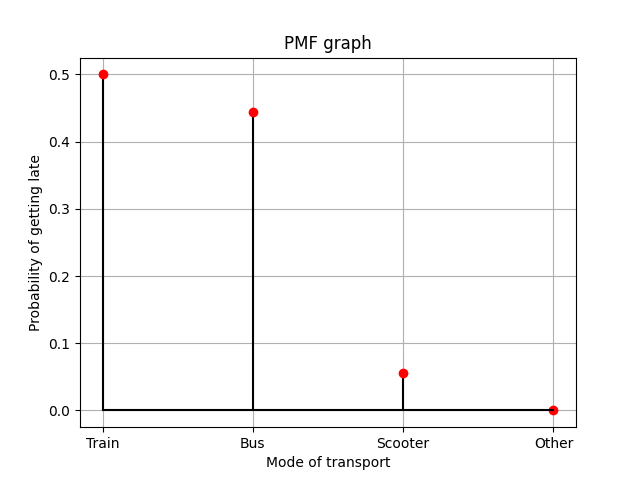
\includegraphics[width=\columnwidth] 
{Figure_1}
\caption{PMF graph }
\label{fig:b}
\end{figure}

\end{document}